\chapter{\textbf{Queueing Network Model}}

The classes of jobs identified in our Queueing Network Model are:
\begin{itemize}
\item StartUp Sampling Water Inland a closed class of job becuase of the deterministic numbers of inland sensors;
\item StartUp Sampling Water Outgoing a closed class of job becuase of the deterministic numbers of Outgoing sensors;
\item Check Water Quality a open class.
\end{itemize}

The first two classes of jobs refer to the same Execution Graph EG UC1, this because of the presence of the case node.
In the diagram below you can see how the jobs interface with our system and how the nodes are interconnected with each other:

\bigskip
\begin{center}
\makebox[\textwidth]{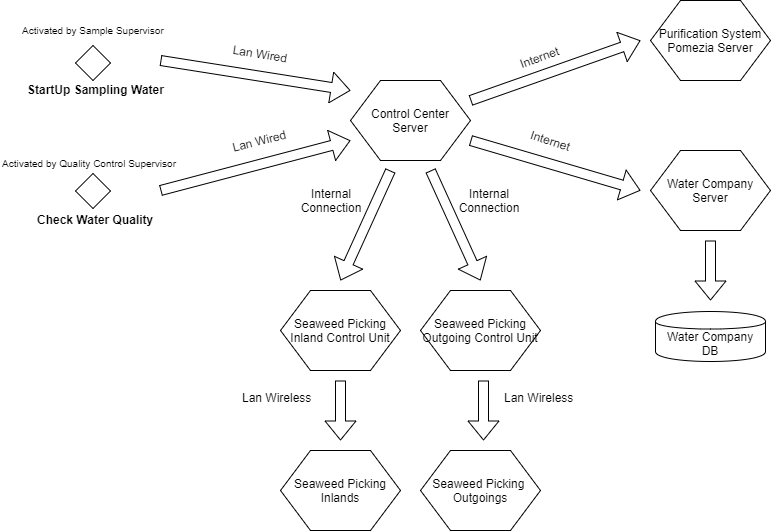
\includegraphics[width= 15cm]				{PhysicalNodes.png}}
\end{center}
\bigskip
\captionof{figure}{Physical Nodes}
\bigskip

This is the Queueing Network so obtained:

\begin{center}
\makebox[\textwidth]{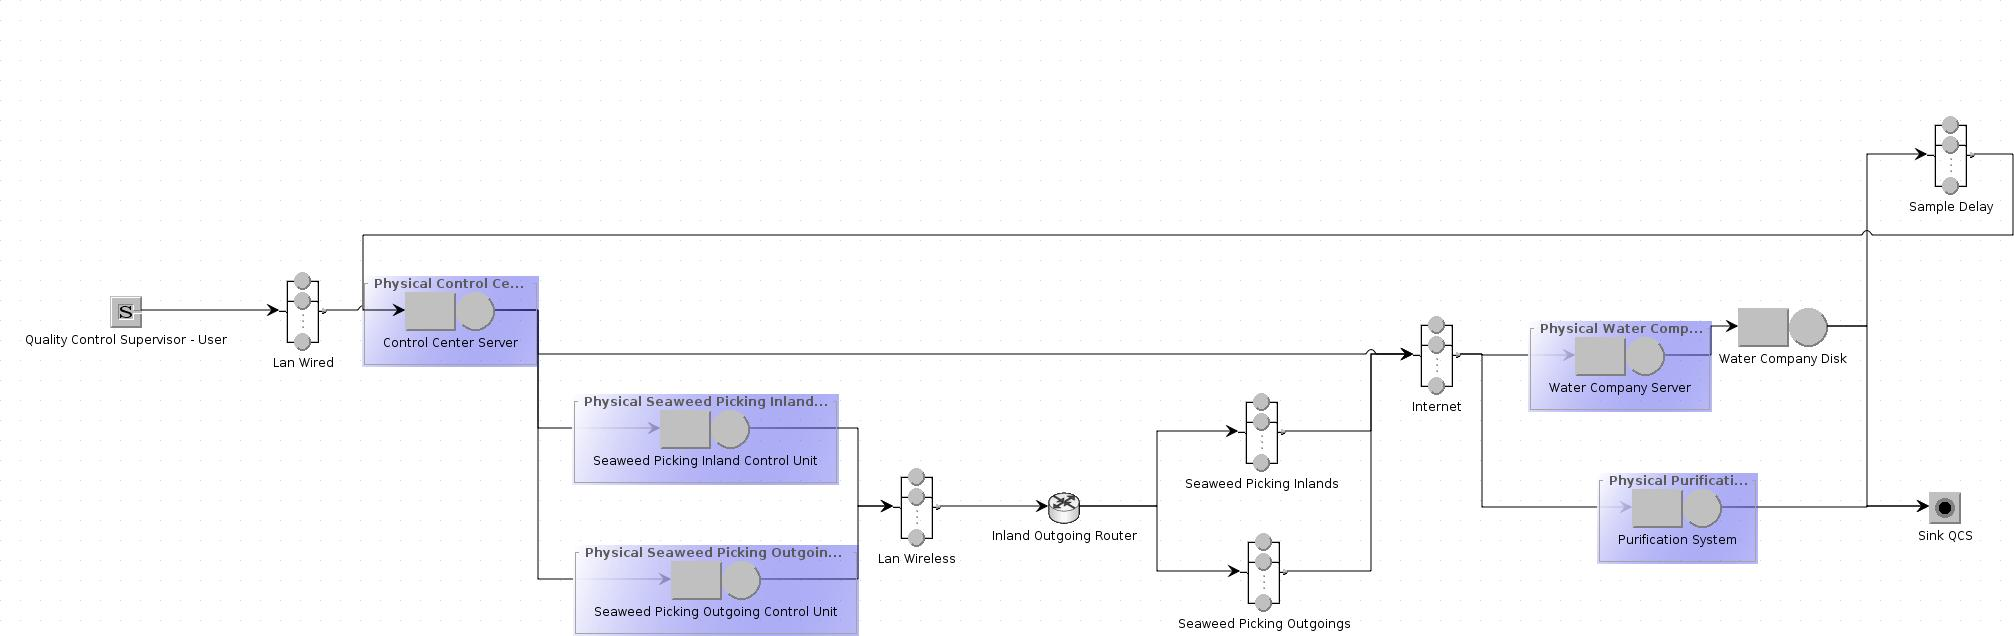
\includegraphics[width=\textwidth]				{QueueingNetwork.jpg}}
\end{center}
\bigskip
\captionof{figure}{Queueing Network}

Below physical nodes will be listed:
\begin{itemize}
\item Computational Nodes;
\begin{itemize}
	\item Control Center Server;
	\item SeaweedPicking Inland Control Unit;
	\item SeaweedPicking Outgoing Control Unit;
	\item Water Company Server;
	\item Purification System.
\end{itemize}
\item Node that store datas:
\begin{itemize}
	\item Water Company Disk.
\end{itemize}	
\item Delay station that simulates Network delays:
\begin{itemize}
	\item Lan Wired;
	\item Lan Wireless;
	\item Internet.
\end{itemize}	
\item Delay station that simulates the sampling:
\begin{itemize}
	\item SeaweedPicking Inlands;
	\item SeaweedPicking Outgoing.
\end{itemize}
\item Delay station that simulates the deterministic interval time 		between sampling of the same Seaweed Picking:
\begin{itemize}
	\item Sample Delay.
\end{itemize}
\end{itemize}

\bigskip
After several tests, in the analysis phase of Chapter 10, we noticed some problems during simulations infact they demanded too long a wait, so we agreed to reduce the sampling time to 100 ms to refine the performance analysis.\\
We have also decided to eliminate the finite capacity regions as useless for the purposes of our project. \\
After other tests we have splitted each StartUp Sampling Water job into:
\begin{itemize}
	\item StartUp Sampling Water;
	\item Sampling.
\end{itemize}
So we obtained the following final calsses of jobs for our Queueing Network: 
\begin{itemize}
	\item StartUp Sampling Water In;
	\item StartUp Sampling Water Out;
	\item Sampling In;
	\item Sampling Out;
	\item Check Water Quality.
\end{itemize}

This choice was driven by the fact that the condition of the loop node in the EG UC1 doesn't specify a deterministic number of repetitions.

\begin{center}
 \makebox[\textwidth]{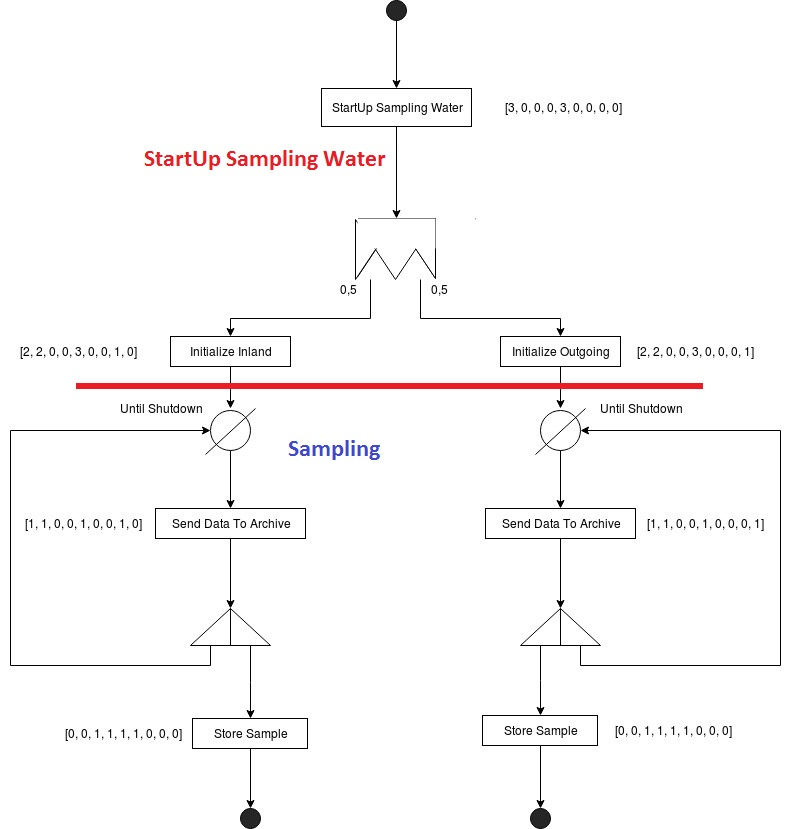
\includegraphics[width=14cm]				{SplittingStartUpSamplingWaterJob.jpg}}
\end{center}
\bigskip
\captionof{figure}{EG UC3 Check Water Quality}
\bigskip

For this purpose a Class Switch Node is introduced where each StartUp Sampling Water becomes a Sampling job.
So our final Queueing Network has become this:
 
\bigskip
\begin{center}
\makebox[\textwidth]{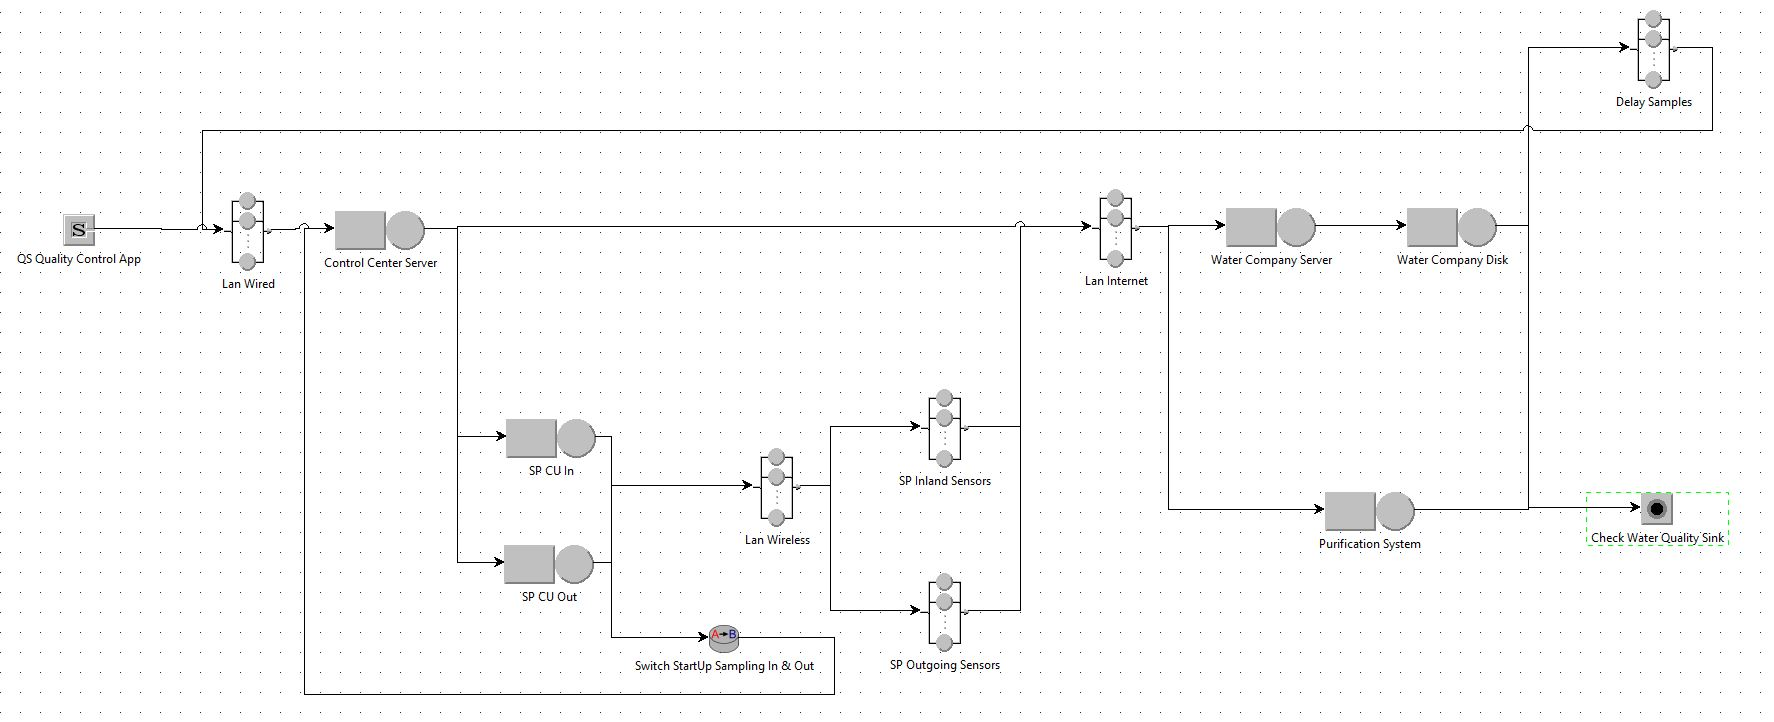
\includegraphics[width= \textwidth]				{QueuingNetworkFinal.jpg}}
\end{center}
\bigskip
\captionof{figure}{Final Queueing Network}



